\chapter{Results}


\section{Elastic properties of particle models}

The numerical relation between macro- and microscopic parameters has been computed for several values of $\interactionRatio$ and compared to the analytical values
\begin{equation}
	\stiffnessTensorElastic =
	\frac{1}{\volume} \sum_\contact \branch^\contact\linkCrossSectionArea^\contact\br{\linkMaterialStiffnessNormal\normalTensor4^\contact+\linkMaterialStiffnessShear\shearTensor4^\contact}
	\label{eqMacroPropertiesElasticTheorStiffnessTensor}
\end{equation}
and
\begin{align}
	\youngModulus &=
	\frac{\sum\branch^\contact\linkCrossSectionArea^\contact}{3\volume}
	\cdot
	\frac{\linkMaterialStiffnessNormal\br{2\linkMaterialStiffnessNormal+3\linkMaterialStiffnessShear}}{4\linkMaterialStiffnessNormal+\linkMaterialStiffnessShear}
	&
	\poissonRatio &= \frac{\linkMaterialStiffnessNormal-\linkMaterialStiffnessShear}{4\linkMaterialStiffnessNormal+\linkMaterialStiffnessShear}
	.
	\label{eqMacroPropertiesElasticTheorElastConstantsApprox}
\end{align}

In graphs, points represent numerically obtained data and data according to analytical estimation of full elastic stiffness tensor.
The line represents the analytical estimation of Young's modulus and Poisson's ratio.

The numerical results of static FEM, quasi-static DEM simulations and analytical full stiffness tensor are practically indistinguishable from each other.
Certain discrepancy can be found for larger values of $\linkMaterialStiffnessShear/\linkMaterialStiffnessNormal\to\infty$ because
then Young's modulus tends to zero relatively to the shear modulus.

As seen from the graphs, the agreement between analytically and numerically obtained data is very good for higher values of $\interactionRatio$.
On the other hand, the analytical formula underestimates the actual (numerically determined) values of Poisson's ratio and overestimates the actual values of Young's modulus for $\interactionRatio<1{.}3$.
For all values of $\interactionRatio$, the value of Poisson's ratio in the limit case for $\linkMaterialStiffnessShear/\linkMaterialStiffnessNormal\to\infty$ ($\linkMaterialStiffnessNormal=0$) is $-1$ (the extreme theoretical value for Poisson's ratio), while the maximum attainable value is $\frac{1}{4}$ for higher values of $\interactionRatio$, which corresponds analytically derive formulas.
A higher value of Poisson's ratio, up to $0{.}335$, is obtained for $\interactionRatio=1{.}05$.

\begin{figure}
	\centering
	\inputplot{preprocessed_macromicro_E_I1.05}
	\inputplot{preprocessed_macromicro_nu_I1.05}
	\\
	\inputplot{preprocessed_macromicro_E_I1.50}
	\inputplot{preprocessed_macromicro_nu_I1.50}
	\caption[Relation between macro- and microscopic parameters]{Relation between macro- and microscopic parameters for $\interactionRatio=1{.}05$ (top) and $\interactionRatio=1{.}50$ (bottom)}
\end{figure}


\section{DEM--FEM coupling}

\subsection{Surface couupling}
This very simple example is aimed to test the approach, mainly correct contact detection and interaction evaluation.
A cantilever is \quotes{bombarded} by three particles.
One particle hits the cantilever \quotes{directly}, while two particles hit the cantilever outside its original position (one aspect of the testing).
The cantilever is modeled by FEM with linear brick elements. The bottom of the cantilever has fixed displacements.
The cantilever surface (set of quadrilateral faces) is triangulated and copied to the DEM part of the simulation.
The DEM \quotes{impactors} can have different shapes, e.g., spherical or polyhedral.
The visual results are shown in figure \ref{figCouplingConcurrentSurfaceExample1}.

\subsection{Volume coupling}
In this example, a simply supported 2D beam subjected to a missile impact was simulated.
The sides of the beam body were simulated by FEM as a plane stress problem using quadrilateral elements linear elastic material law.
The central part was modeled by DEM using a regular packing and CPM material model.
The material parameters and initial conditions are artificially set to get \quotes{nice} results.
The visual results are shown in figure \ref{figCouplingConcurrentVolumeExample1}.

\subsection{Multiscale coupling}
Uniaxial strain (oedometric test) of a sample consisting of three different (linear elastic) materials is simulated in this example.
The macro-scale problem is modeled by three brick elements.
Each FEM element has eight integration points.
The upper one is a pure FEM element.
For each integration point of the two bottom elements, different DEM micro-scale RVE simulations are performed.

The visual results are shown in figure \ref{figCouplingConcurrentMultiExample1}.
In each \quotes{DEM} element, one micro RVE result is displayed.
The results of linear elastic behavior are not extremely spectacular indeed, but using a nonlinear behavior of RVEs (resulting in a higher stiffness when more inter-particle contacts occur for instance) could be very useful for certain applications.

\subsection{Contact coupling}

In this example, collision of three elastic bodies is presented.
All three particles are modeled by FEM, only a detection algorithm is borrowed from DEM.
The visual results are shown in figure \ref{figCouplingConcurrentContactExample1}.

\begin{figure}[p]
	\centering
	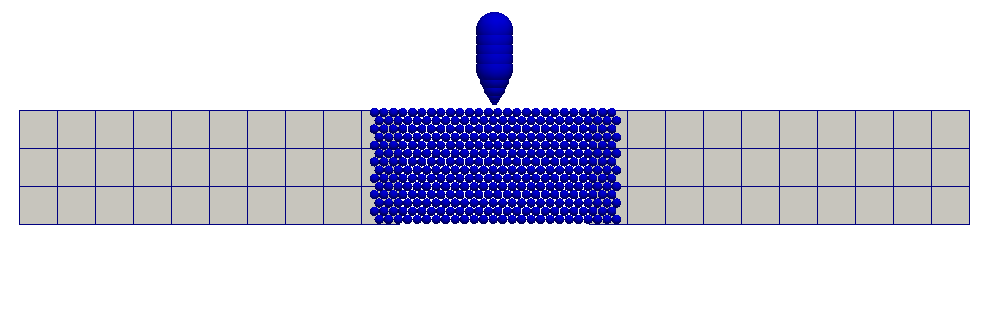
\includegraphics[width=15cm,trim={0 3.5cm 0 0cm},clip]{coupling/vol1/vol1-0000}
	\\
	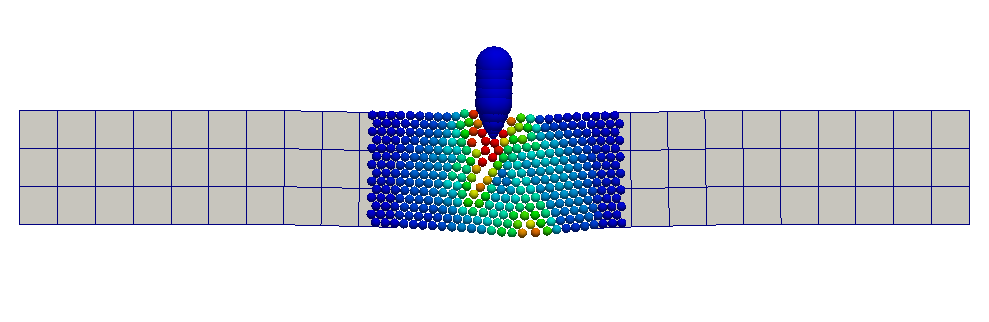
\includegraphics[width=15cm,trim={0 2.5cm 0 1.5cm},clip]{coupling/vol1/vol1-0020}
	\\
	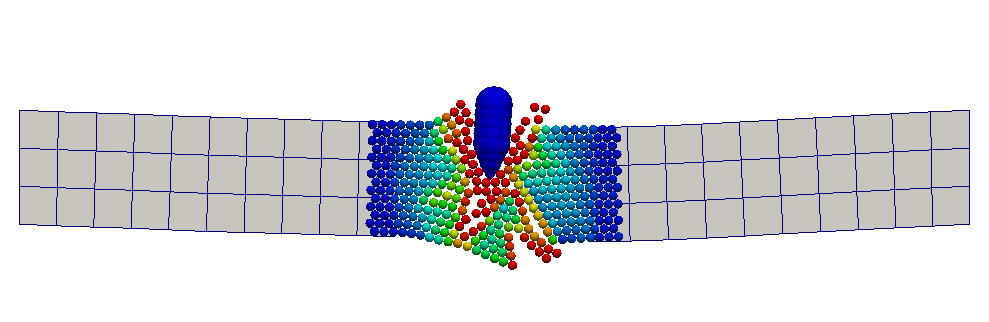
\includegraphics[width=15cm,trim={0 1.5cm 0 2.5cm},clip]{coupling/vol1/vol1-0050}
	\\
	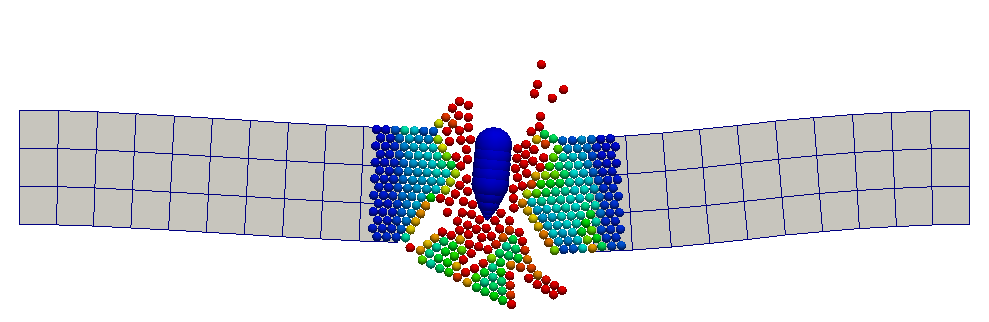
\includegraphics[width=15cm,trim={0 .0cm 0 2cm},clip]{coupling/vol1/vol1-0087}
	\caption{Impact on a simply supported beam at different stages}
	\label{figCouplingConcurrentVolumeExample1}
\end{figure}

\begin{figure}[p]
	\centering
	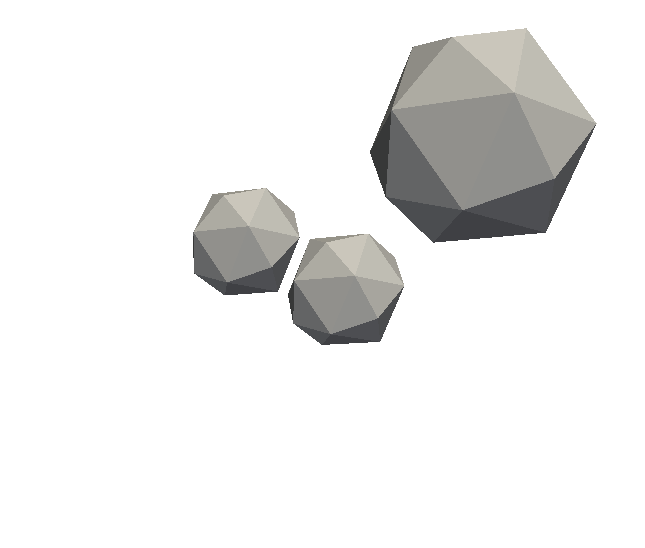
\includegraphics[width=5cm]{coupling/contact1/contact1-0010}
	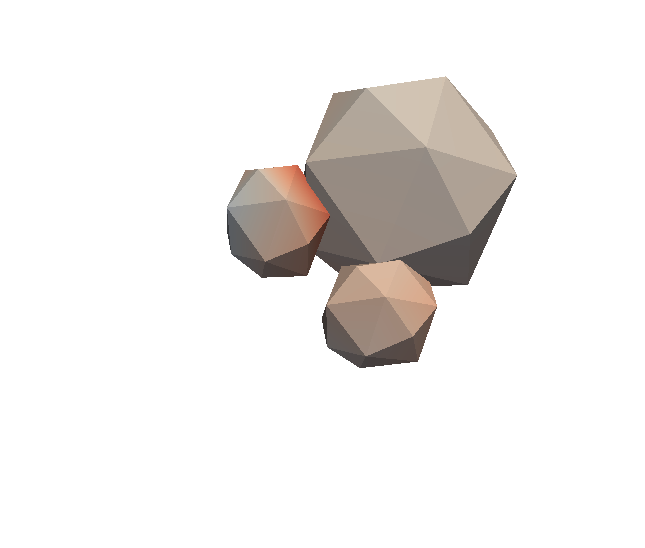
\includegraphics[width=5cm]{coupling/contact1/contact1-0053}
	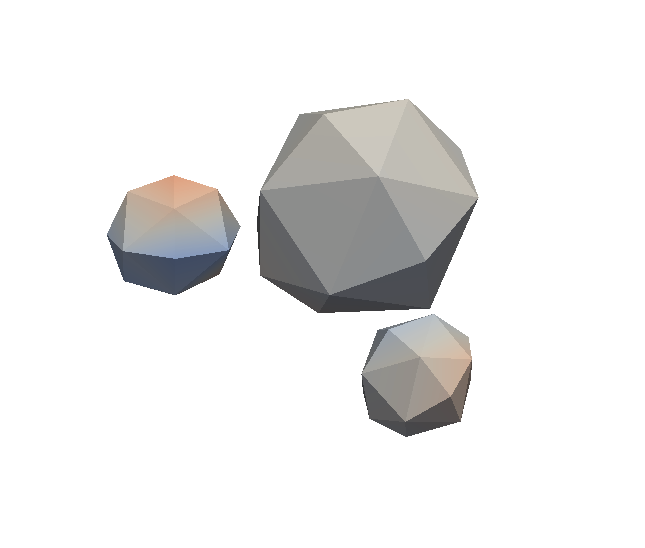
\includegraphics[width=5cm]{coupling/contact1/contact1-0080}
	\caption{Collision of three elastic particles at different stages}
	\label{figCouplingConcurrentContactExample1}
\end{figure}

\begin{figure}[p]
	\centering
	\includegraphics[width=5cm]{coupling/surf1/spheres/surf1-0000}
	\includegraphics[width=5cm]{coupling/surf1/spheres/surf1-0030}
	\includegraphics[width=5cm]{coupling/surf1/spheres/surf1-0060}
	\\
	\includegraphics[width=5cm]{coupling/surf1/poly/surf1-0000}
	\includegraphics[width=5cm]{coupling/surf1/poly/surf1-0030}
	\includegraphics[width=5cm]{coupling/surf1/poly/surf1-0060}
	\caption[Impact on a cantilever at different stages]{Impact on a cantilever at different stages. DEM particles can be spheres (top) or polyhedrons (bottom).}
	\label{figCouplingConcurrentSurfaceExample1}
\end{figure}

\begin{figure}[p]
	\centering
	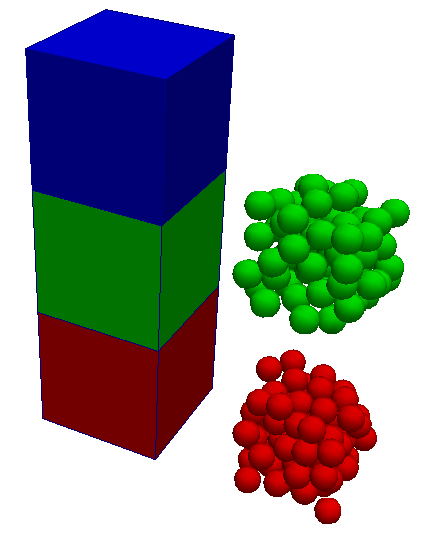
\includegraphics[width=5cm]{coupling/multi1/multi1-0000}
	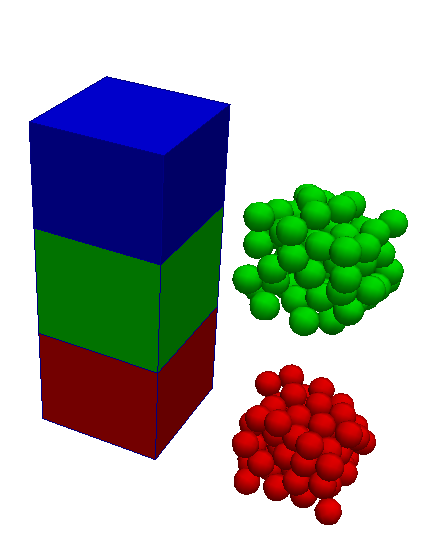
\includegraphics[width=5cm]{coupling/multi1/multi1-0025}
	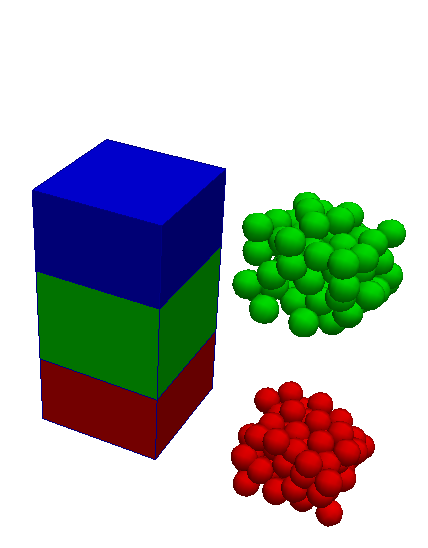
\includegraphics[width=5cm]{coupling/multi1/multi1-0050}
	\caption{Uniaxial strain test at different stages}
	\label{figCouplingConcurrentMultiExample1}
\end{figure}



\section{Sequential coupling - uniaxial compression}\label{secCouplingSequentialExamples}
In this section, the results of proposed sequential coupling method are shown on simple \quotes{one element} tests.
The simulated prismatic specimen is subjected to uniaxial compression.
In the case of a one-element FEM simulation, the definition of boundary conditions is straightforward.
In~the DEM simulation, the axial strain is imposed by prescribed displacements at the top and bottom boundary layers.
In the lateral directions, the particles are free to move.
For the graphical post-processing, the stress values from DEM simulation are obtained as the normal component in the axial direction of the average stress.

The DEM and FEM material parameters are set such that the resulting stress-strain diagrams are as similar as possible.
Figure \ref{figCouplingSequantialResultsMapping} shows a very good agreement of the two models in both pre-peak and post-peak regime.
However, the two models differ at the peak load (the CPM softening starts prior to the DPM softening).

The DEM specimen is loaded at a certain level and then possibly unloaded.
At the final stage of the DEM simulation, relevant quantities are mapped onto the one-element FEM simulation and the FEM simulation is run.
The average stress tensor and average damage tensor are evaluated from all \quotes{ordinary} particles (not belonging to the layer imposing boundary conditions).

Graphs in figures \ref{figCouplingSequantialResultsMapping} show results of the CPM simulation (grey) and continuation with the mapped DPM model (black).
The presented results show a reasonable approximation of the FEM behavior after the transformation from DEM.
The biggest error is obtained, if the mapping occurs around the peak (or after unloading from around the peak) where the results of two presented models differ the most.

\begin{figure}
	\centering
	\inputplot{sequential_coupling_plain}
	\inputplot{sequential_coupling_002}
	\inputplot{sequential_coupling_004}
	\inputplot{sequential_coupling_005}
	\inputplot{sequential_coupling_007}
	\inputplot{sequential_coupling_009}
	\caption{Results of sequential coupling}
	\label{figCouplingSequantialResultsMapping}
\end{figure}







\section{Discrete mesoscale model for concrete - experiment \cite{BeygiEtAl2014a,BeygiEtAl2014b,NikbinEtAl2014a}}

From the studied literature, the experiment from \cite{BeygiEtAl2014a,BeygiEtAl2014b,NikbinEtAl2014a} was chosen for validation.
The experiments investigate the influence of different aggregate sizes (different grading curves) on concrete material properties ($f_t$, $f_c$, $G_f$, $E$).
Two concrete compositions (low strength and high strength) are examined, each with three different aggregate grading curves.

Figures \ref{figMCPMValidation} show the comparison between simulations and experimental data.
Since the absolute values of macroscopic quantities can be relatively easily estimated, only values relative to the results for the smallest aggregate size are plotted.

Each point in the graphs is the averaged simulation result from 3 runs.
For each run, the same aggregate sizes were considered (according to the corresponding concrete composition and grading curve) and their positions were chosen randomly.
The simulations were performed on 50 mm cubic samples with 2 mm DEM particle size (diameter).

Several combinations of input parameters were tested. The results are plotted for
aggregates 2.5 time stiffer and 5 time stronger than matrix
and for
ITZ 2 times less stif and 2 times weaker than mortar links.
Results 2 refer to 2 times more brittle ITZ than results 1.

The model results reasonably correspond to the trends observed in the experiments, although the precise values are fitted with a certain discrepancy.

\begin{figure}[htbp]
	\centering
	\resizebox{!}{.25\textheight}{\inputplot{validationBeygi_l}}
	\resizebox{!}{.25\textheight}{\inputplot{validationBeygi_h}}
	\caption[Comparison of simulations and experiment]{Comparison of simulations and experiment \cite{BeygiEtAl2014a,BeygiEtAl2014b,NikbinEtAl2014a} for low strength (top) and high strength (bottom) concrete.}
	\label{figMCPMValidation}
\end{figure}
